%\documentclass[iop]{emulateapj}
\documentclass[preprint]{aastex}
%\documentclass[12pt, onecolumn]{emulateapj}
%\documentstyle[aas2pp4,natbib209]{article}

\usepackage{tikz}
\usepackage{natbib}
\usepackage{amsmath}

\usetikzlibrary{shapes.geometric, arrows}
\usetikzlibrary{fit}

\tikzstyle{hyper} = [circle, text centered, draw=black]
\tikzstyle{param} = [circle, text centered, draw=black]
\tikzstyle{data} = [circle, text centered, draw=black, line width=2pt]
\tikzstyle{arrow} = [thick,->,>=stealth]

\newcommand{\myemail}{aimalz@nyu.edu}
\newcommand{\textul}{\underline}

\shorttitle{How to obtain the redshift distribution from probabilistic redshift estimates}
\shortauthors{Malz and Hogg}

\begin{document}

\title{How to obtain the redshift distribution from probabilistic redshift estimates}

\author{Alex Malz\altaffilmark{1} \& David W. Hogg\altaffilmark{1,2,3,4}}
\email{aimalz@nyu.edu}

\altaffiltext{1}{Center for Cosmology and Particle Physics, Department of Physics,
  New York University, 726 Broadway, 9th floor, New York, NY 10003, USA}
\altaffiltext{2}{Simons Center for Computational Astrophysics, 162 Fifth Avenue, 7th floor, New York, NY 10010, USA}
\altaffiltext{3}{Center for Data Science, New York University, 60 Fifth Avenue, 7th floor, New York, NY 10003, USA}
\altaffiltext{4}{Max-Planck-Institut f\"ur Astronomie, K\"onigstuhl 17, D-69117 Heidelberg, Germany}

\begin{abstract}
The redshift distribution $n(z)$ is a crucial ingredient for weak lensing cosmology.  Spectroscopically confirmed redshifts for the dim and numerous galaxies observed by weak lensing surveys are expected to be inaccessible, making photometric redshifts (photo-$z$s) the next best alternative.  Because of the nontrivial inference involved in their determination, photo-$z$ point estimates are being superseded by photo-$z$ probability distribution functions (PDFs).  However, analytic methods for utilizing these new data products in cosmological inference are still evolving.

This paper presents a novel approach to estimating the posterior distribution over $n(z)$ from a survey of galaxy photo-$z$ PDFs based upon a probabilistic graphical model of hierarchical inference.  We present the Cosmological Hierarchical Inference with Probabilistic Photometric Redshifts (CHIPPR) code implementing this technique, as well as its validation on mock data and testing on a subset of BOSS DR10.  CHIPPR yields an accurate characterization of $n(z)$ containing information beyond the best-fit estimator produced by traditional procedures.  The publicly available code is easily extensible to other one-point statistics that depend on redshift.

\end{abstract}

\keywords{catalogs --- cosmology: cosmological parameters --- galaxies: statistics --- gravitational lensing: weak --- methods: analytical --- methods: data analysis --- methods: statistical --- techniques: photometric}

\section{Introduction}
\label{sec:introduction}

The redshift distribution $n(z)$ is necessary for calculating two-point statistics of galaxy properties used to determine the cosmological parameter values that inform our understanding of the evolution of large-scale structure in the universe \citep{masters_mapping_2015}.  Inaccurate estimates of $n(z)$ can significantly impact the constraining power of a galaxy survey, biasing recovery of the cosmological parameters.  For example, if the $n(z)$ used in analysis is offset from the true $n(z)$ by a small, negative constant, it results in underestimating $w_{0}$ and overestimating $\sigma_{8}$ \citep{samuroff_simultaneous_2017}.

Though the redshift density function has traditionally been determined from spectroscopically observed redshifts, modern galaxy surveys including DES, LSST, Euclid, and WFIRST seek to obtain two-point statistics of redshift from samples of galaxies for which spectroscopic redshifts are unavailable, either due to their large numbers or their low brightnesses.  For decades, photometrically estimated redshifts (photo-$z$s) have been the leading alternative to spectroscopically observed redshifts, though they suffer from issues of precision in the form of an intrinsic scatter and accuracy in the form of catastrophic outliers, as well as other systematics imparted by the properties of the survey, data reduction pipeline(s), and assumptions underlying the analysis \citep{baum_photoelectric_1962}.  These weaknesses are illuminated by a probabilistic interpretation of photo-$zs$; if these nontrivial uncertainties were expressed as a probability distribution function (PDF) over redshift, photo-$z$s could be replaced by photo-$z$ PDFs containing more information than a simple point estimate \citep{koo_overview_1999}.  Such data products have been commonly released by photometric galaxy surveys since SDSS DR7 \citep{abazajian_seventh_2009} using a great variety of methods.

Methods for using photo-$z$ PDFs in cosmological inference remain underdeveloped, with many survey pipelines reducing them to familiar point estimators that are compatible with existing technology or engaging with them heuristically in a manner inconsistent with their probabilistic nature.  Stacking photo-$z$ PDFs, or other mathematically equivalent methods, to obtain an estimator of $n(z)$ is especially popular \citep{cunha_estimating_2009, sheldon_photometric_2012}.  However, photo-$z$ PDFs are probabilistic data products that must be handled in a fully consistent, probabilistic manner; hierarchical inference is the only mathematically valid way to do inference with photo-$z$ PDFs and other probabilistic quantities.

It is desirable to create rigorous methods for using photo-$z$ PDFs in inference, beginning with the simplest one-point statistic of redshift, $n(z)$.  In the spirit of \citet{hogg_inferring_2010, foreman-mackey_exoplanet_2014}, this paper derives a mathematically rigorous approach to inferring $n(z)$ in Sec. \ref{sec:method}.  The presentation of a public code implementing this novel technique is given in Sec. \ref{sec:model_specifics}.  The code is validated on mock data and tested on a subset of BOSS DR10 data in Sec. \ref{sec:experiments}.  We conclude and discuss future directions in Sec. \ref{sec:discussion}.

\section{Method}
\label{sec:method}

The redshift distribution $n(z)$ may be understood as the probability of finding a galaxy at a redshift $z$.  We may express $n(z)$ in terms of some functional form $f_{\vec{\theta}}(z)$ with parameters comprising $\vec{\theta}$ according to Eq. \ref{eq:parametrization}.  
\begin{align}
\label{eq:parametrization}
n(z) &\equiv f_{\vec{\theta}}(z)\ \equiv\ p(z|\vec{\theta})
\end{align}
In this work, we wish to characterize the posterior distribution $p(\vec{\theta}|\textul{D})$ of the parameters contained in $\vec{\theta}$ defining $n(z)$ given all available data $\textul{D}$.  The likelihood $p(z|\vec{\theta})$ represents the probability of a random variable, in this case redshift $z$, given the parameters in $\vec{\theta}$ defining the distribution $n(z)$ from which it is drawn.  Our model for inferring $p(\vec{\theta}|\textul{D})$ will be introduced in Sec. \ref{sec:derivation}, and alternative methods of estimating $\vec{\theta}$ will be presented in Sec. \ref{sec:alternatives}.

\subsection{Derivation}
\label{sec:derivation}

Inference of $p(\vec{\theta}|\textul{D})$ is perfectly suited to a hierarchical Bayesian model.  In this problem, the available data $\textul{D}$ is a catalog of photometry $\{\vec{d}_{i}\}$ of individual galaxies $i$ where each $\vec{d}_{i}$ is a random variable that is a function of its redshift parameter $z_{i}$; the redshift parameters $\{z_{i}\}$ are independently drawn from a function defined by hyperparameters in $\vec{\theta}$.  These physical relationships may be illustrated in Fig. \ref{fig:pgm} by a directed acyclic graph representing a probabilistic graphical model (PGM).
\begin{figure}
\begin{center}
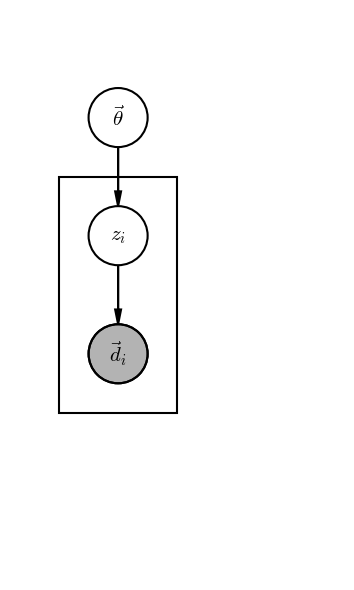
\includegraphics[width=0.5\textwidth]{pgm.png}
\caption{This directed acyclic graph corresponds to a PGM for a hierarchical inference of $p(\vec{\theta}|\{\vec{d}_{i}\})$.  In this graph, all random variables are shown in circles, with observed variables shown in shaded circles.  Relationships between variables are indicated by arrows.  The box indicates that there are a number of copies of the relationships between boxed parameters, each independent of all others.  The hyperparameters $\vec{\theta}$ representing $n(z)$ are at the top.  Independently drawn from a function of the hyperparameters $\vec{\theta}$ are galaxy redshifts $\{z_{i}\}$ below.  The observed galaxy photometry $\{\vec{d}_{i}\}$, shown in shaded circles, is determined by the redshifts above.}
\label{fig:pgm}
\end{center}
\end{figure}
This PGM may be used as the basis for a derivation of the desired hyperposterior $p(\vec{\theta}|\{\vec{d}_{i}\})$, assuming our physical model is complete.  From this point on, we will work solely with log probabilities.

We begin with Eq. \ref{eq:hyperbayes} by applying Bayes' Rule to express the log-hyperposterior $\ln\left[p(\vec{\theta}|\{\vec{d}_{i}\})\right]$ in terms of the log-hyperlikelihood $\ln\left[p(\{\vec{d}_{i}\}|\vec{\theta})\right]$.
\begin{align}
\label{eq:hyperbayes}
\ln\left[p(\vec{\theta}|\{\vec{d}_{i}\})\right] &\propto \ln\left[p(\vec{\theta})\right] + \ln\left[p(\{\vec{d}_{i}\}|\vec{\theta})\right]
\end{align}
To do this, we will choose a log-hyperprior distribution $\ln\left[p(\vec{\theta})\right]$ representing our beliefs about the distribution of the hyperparameters $\vec{\theta}$ in terms of fixed variables that we will assume are known.

The log-hyperlikelihood $\ln\left[p(\{\vec{d}_{i}\}|\vec{\theta})\right]$ contains no explicit reference to redshifts, therefore, we employ the PGM to write the marginalization over the redshifts in Eq. \ref{eq:marginalization}.
\begin{align}
\label{eq:marginalization}
\ln\left[p(\{\vec{d}_{i}\}|\vec{\theta})\right] &= \ln\left[\int\ p(\{\vec{d}_{i}\}|\{z_{i}\})\ p(\{z_{i}\}|\vec{\theta})\ d\{z_{i}\}\right]
\end{align}
We shall handle the two terms in the integral separately.

The first term is the likelihood of all galaxy photometry given all galaxy redshifts.  If we assume independence of galaxy photometry, such that $p(\vec{d}_{i}|\{\vec{d}_{i'\neq i}\}, \{z_{i}\})=p(\vec{d}_{i}|z_{i})$, then we may write Eq. \ref{eq:independentdata}.
\begin{align}
\label{eq:independentdata}
\ln\left[p(\{\vec{d}_{i}\}|\{z_{i}\})\right] &= \sum_{i}\ln\left[p(\vec{d}_{i}|z_{i})\right]
\end{align}
The second term may also be expanded as in Eq. \ref{eq:independentredshifts} by assuming that all galaxy redshifts are drawn independently from $n(z)$.
\begin{align}
\label{eq:independentredshifts}
\ln\left[p(\{z_{i}\}|\vec{\theta})\right] &= \sum_{i}\ln\left[p(z_{i}|\vec{\theta})\right]
\end{align}
Since all galaxy redshifts are independent of one another, an integral over the aggregate $\int\dots d\{z_{i}\}$ is simply the product of the integrals over each one $\prod_{i}\int\dots dz_{i}$.  Thus, the log-hyperlikelihood can be written according to Eq. \ref{eq:log-hyperlikelihood}.
\begin{align}
\label{eq:log-hyperlikelihood}
\ln\left[p(\{\vec{d}_{i}\}|\vec{\theta})\right] &= \sum_{i}\ln\left[\int\ p(\vec{d}_{i}|z_{i})\ p(z_{i}|\vec{\theta})\ dz_{i}\right]
\end{align}
The expression of Eq. \ref{eq:log-hyperlikelihood} contains two types of quantities.  The $\{p(z_{i}|\vec{\theta})\}$ are known likelihoods that will be equal to $\{f_{\vec{\theta}}(z_{i})\}$.  The $\{p(\vec{d}_{i}|z_{i})\}$, however, are likelihoods that are unknown and in general unknowable, and it is worth discussing these facts.  

Photo-$z$ PDFs are commonly written simply as $p(z)$, but this notation oversimplifies their substance.  Whether determined by way of template-fitting or machine learning, photo-$z$ PDFs are dependent on the data $\vec{d}$ from which they are calculated.  This data $\vec{d}$ must be considered to be a quantity upon which the redshift $z$ is conditioned, otherwise normalizing a photo-$z$ PDF would require integrating over all possible values of $\vec{d}$.  This means that photo-$z$ PDFs are posteriors, probabilities of parameters $z$ conditioned on data $\vec{d}$.  However, where there is a posterior, there is always a prior.  Photo-$z$ PDFs are in general \textit{interim} posteriors, because in addition to being conditioned on observations, they are also conditioned on an interim prior in the form of a particular value $\vec{\theta}^{*}$ of $\vec{\theta}$ necessary for computing the photo-$z$ PDF.  In the case of template-fitting methods, the interim prior is usually specified as an input to the photo-$z$ PDF production code, and it often takes the form of an initial guess for $\vec{\theta}$ based on the results of previous galaxy surveys or simulations thereof; in the case of machine learning methods, the interim prior may be explicitly derived from the training set or implicitly produced in the process of determining the photo-$z$ PDFs, and the interim prior is not always revealed to the user.   Hierarchical inference may be performed only when the interim prior is known, which means it will only be possible for photo-$z$ PDFs made via certain methods.

Since the data products from which we hope to probe the log-hyperposterior are themselves posteriors, we must express the likelihoods $\{p(\vec{d}_{i}|z_{i})\}$ of Eq. \ref{eq:log-hyperlikelihood} in terms of the photo-$z$ PDFs $\{p(z_{i}|\vec{d}_{i}, \vec{\theta}^{*})\}$.  We start by multiplying the likelihood by an inspired factor of unity written in terms of the photo-$z$ interim posterior we have at hand, as in Eq. \ref{eq:unity}.
\begin{align}
\label{eq:unity}
p(\vec{d}_{i}|z_{i}) &= p(\vec{d}_{i}|z_{i})\ \frac{p(z_{i}|\vec{d}_{i}, \vec{\theta}^{*})}{p(z_{i}|\vec{d}_{i}, \vec{\theta}^{*})}
\end{align}
Next, we expand the denominator in terms of Bayes' Rule to obtain Eq. \ref{eq:bayes}.
\begin{align}
\label{eq:bayes}
p(\vec{d}_{i}|z_{i}) &= p(\vec{d}_{i}|z_{i})\ p(z_{i}|\vec{d}_{i}, \vec{\theta}^{*})\ \frac{p(\vec{d}_{i}|\vec{\theta}^{*})}{p(z_{i}|\vec{\theta}^{*})\ p(\vec{d}_{i}|z_{i}, \vec{\theta}^{*})}
\end{align}
Because the redshift $z_{i}$ is independent of the interim prior $\vec{\theta}^{*}$, the interim likelihood $p(\vec{d}_{i}|z_{i}, \vec{\theta}^{*})$ may be expanded further as in Eq. \ref{eq:expansion}.
\begin{align}
\label{eq:expansion}
p(\vec{d}_{i}|z_{i}) &= p(\vec{d}_{i}|z_{i})\ p(z_{i}|\vec{d}_{i}, \vec{\theta}^{*})\ \frac{p(\vec{d}_{i}|\vec{\theta}^{*})}{p(z_{i}|\vec{\theta}^{*})\ p(\vec{d}_{i}|z_{i})\ p(\vec{d}_{i}|\vec{\theta}^{*})}
\end{align}
We cancel the terms $p(\vec{d}_{i}|z_{i})$ and $p(\vec{d}_{i}|\vec{\theta}^{*})$ that appear in both the numerator and denominator of Eq. \ref{eq:expansion} to obtain Eq. \ref{eq:cancellation}.
\begin{align}
\label{eq:cancellation}
p(\vec{d}_{i}|z_{i}) &= \frac{p(z_{i}|\vec{d}_{i}, \vec{\theta}^{*})}{p(z_{i}|\vec{\theta}^{*})}
\end{align}

Finally we may return to Eq. \ref{eq:hyperbayes} to express the log-hyperposterior $\ln\left[p(\vec{\theta}|\{\vec{d}_{i}\})\right]$ in terms of the photo-$z$ interim posteriors $\{p(z_{i}|\vec{d}_{i}, \vec{\theta}^{*})\}$, as in Eq. \ref{eq:final}.
\begin{align}
\label{eq:final}
\ln\left[p(\vec{\theta}|\{\vec{d}_{i}\})\right] &\propto \ln\left[p(\vec{\theta})\right] + \sum_{i}\ln\left[\int\ p(z_{i}|\vec{d}_{i}, \vec{\theta}^{*})\ \frac{p(z_{i}|\vec{\theta})}{p(z_{i}|\vec{\theta}^{*})}\ dz_{i}\right]
\end{align}
Now we have an expression for a quantity proportional to the log-hyperposterior we desire!  Though the constant of proportionality, $p(\{\vec{d}_{i}\})$ is in general not possible to calculate, we may still characterize the log-hyperposterior by way of MCMC sampling and optimization, which will be discussed in Sec. \ref{sec:implementation}.

Several assumptions were noted in the above derivation; for clarity, they will be enumerated below, where their limitations will be discussed.
\begin{enumerate}
\item The PGM is an expression of our beliefs about the physics of the problem, and the inference will only be valid to the degree that the model is correct.  One can easily think of ways in which the PGM of Fig. \ref{fig:pgm} is incomplete; for example, intrinsic galaxy SEDs will evolve with redshift.  However, we assume that physical processes not represented in the PGM of Fig. \ref{fig:pgm} are subdominant and may thus be neglected.
\item We must choose a hyperprior $p(\vec{\theta})$; we assume that our choice of a sufficiently general hyperprior that will not be a dominant source of information in the hyperposterior is successful.  If we choose poorly, the hyperprior may dominate over the hyperlikelihood, downweighting the significance of the data in determining the hyperposterior or biasing the result based on a misunderstanding of the underlying physics.
\item We assume independence of galaxies in our catalog such that each galaxy's photometry $\vec{d}_{i}$ is independent from all other galaxies' photometry $\{\vec{d}_{i'\neq i}\}$ and all other galaxies' redshifts $\{z_{i'\neq i}\}$.  However, the photometry $\{\vec{d}_{i}\}$ will inherently share instrumental and systematic effects due to being observed with the same telescope as part of a single survey project.  Furthermore, there may be blended objects or other correlations between the redshifts of different galaxies.  We must assume that such effects are negligible and will not consider them in this treatment.  
\item We assume that the interim prior is known to us, either as input to or output of the method producing the photo-$z$ interim posteriors.  Furthermore, it must be representable in the parametrization of $f_{\vec{\theta}}(z)$, i.e. our model $f_{\vec{\theta}}(z)$ for $n(z)$ must be flexible enough to encompass both the true distribution we aim to probe and the interim prior.
\item Finally, we assume that the photo-$z$ interim posteriors $\{p(z_{i}|\vec{d}_{i}, \vec{\theta}^{*})\}$ are accurate.  There is some evidence that photo-$z$ PDFs derived by different methods disagree with one another or are strongly dependent on the interim prior.  However, the choice of the technique by which the photo-$z$ interim posteriors are determined is outside the scope of this paper.
\end{enumerate}

\subsection{Alternative methods}
\label{sec:alternatives}

This method is presented in contrast to existing methods for inferring $n(z)$ from photo-$z$ PDFs, which fall into two broad categories: stacking and point estimation.  Stacking assumes Eq. \ref{eq:stacking}, where the constant of proportionality is chosen to ensure $\int f_{\vec{\theta}}(z)\ dz$ is unity.
\begin{align}
\label{eq:stacking}
f_{\vec{\theta}}(z) &\propto \sum_{i}p(z_{i}|\vec{d}_{i}, \vec{\theta}^{*})
\end{align}

\section{Implementation}
\label{sec:implementation}

We introduce the Cosmological Hierarchical Inference with Probabilistic Photometric Redshifts (CHIPPR) code as a comprehensive package for estimating $n(z)$ from catalogs of photo-$z$ PDFs.  In particular, CHIPPR implements both sampling and optimization of Eq. \ref{eq:final} and compares the results to those of the more traditional approaches presented in Sec. \ref{sec:alternatives}.

\section{Experiments}
\label{sec:experiments}

\section{Discussion}
\label{sec:discussion}

%\appendix{}

\begin{acknowledgements}
AIM thanks Phil Marshall for advising on the production of usable code, Mohammadjavad Vakili for insightful input on statistics, Geoffrey Ryan for assistance in debugging code, and Boris Leistedt for helpful comments provided in the preparation of this paper.
\end{acknowledgements}

\bibliographystyle{apj}
\bibliography{references}

\end{document}